\begin{figure}[htbp]
\centering
\begin{tikzpicture}[x=1cm,y=1cm]
\node[anchor=south west,inner sep=0] at (0,0) {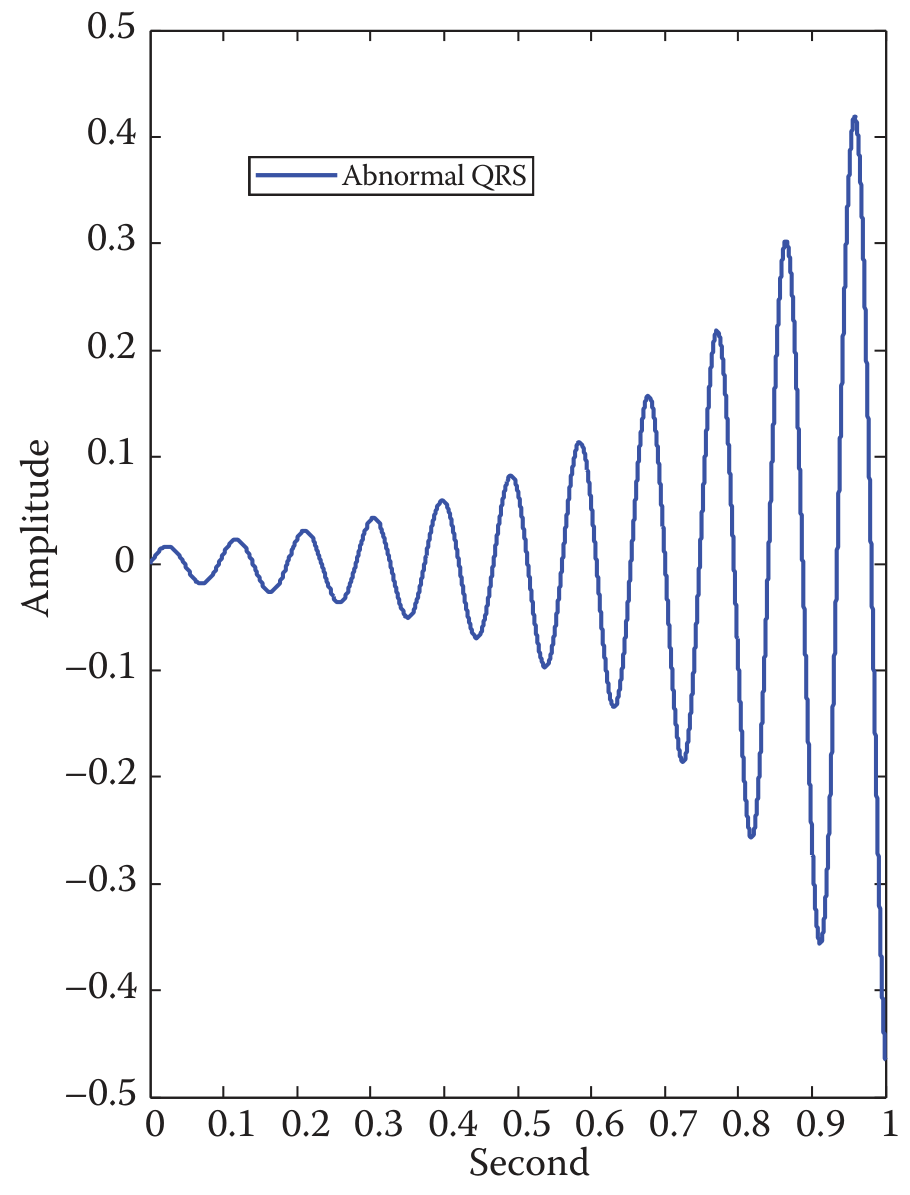
\includegraphics[width=9.0cm]{figures/ch03_fig05_data.png}};
\fill[white] (3.3626,9.9148) rectangle (5.2418,10.2412);
\fill[white] (4.6029,0.0749) rectangle (5.8648,0.5199);
\node[font=\scriptsize,rotate=0,inner sep=0] at (5.2339,0.2974) {时间（秒）};
\fill[white] (0.1459,5.6806) rectangle (0.6008,7.5043);
\node[font=\scriptsize,rotate=90,inner sep=0] at (0.3733,6.5924) {振幅};
\node[font=\scriptsize,rotate=0,inner sep=0] at (4.2946,10.0599) {异常 QRS};
\end{tikzpicture}
\origfig{5}{正常 QRS 波群所对应心脏系统的单位阶跃响应曲线。}
\label{fig:ch03-05}
\end{figure}
